\section{Experimental Results}

\subsection{Simulated Runs}
We simulated performance of our algorithms on random graphs generated
by the graph models we outlined. In the following figures, each data
point is obtained by averaging the measurements over 10 random
graphs. We first present the time and space usage of these algorithms when
solving a $(3,3)$-recommendation subgraph problem in different sized graphs.
Note that varying the value of $a$ and $c$ would only change space and time
usage by a constant, so these two graphs are indicative of time and space
usage over all ranges of parameters

\begin{figure}[t]
\centering
\begin{minipage}[h]{0.48\textwidth}
\centering
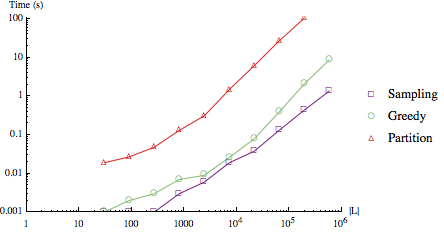
\includegraphics[width=0.8\textwidth]{images/time.png}
\caption{Time needed to solve a (3,3)-recommendation problem in random graphs where $|L|$ scales as $|R|$ with k=4.}\label{fig:time_graph}
\end{minipage}
\hspace{0cm}
\begin{minipage}[h]{0.48\textwidth}
\centering
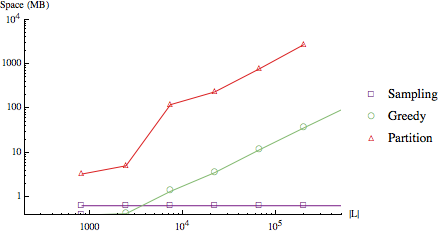
\includegraphics[width=0.8\textwidth]{images/space.png}
\caption{Space needed to solve a (3,3)-recommendation problem in random graphs where $|L|$ scales as $|R|$ with k=4.}\label{fig:space_graph}
\end{minipage}
\vspace{-0.2in}
\end{figure}
\vs

Recall that the partition algorithm split the graph into multiple graphs
and found matchings in these smaller graphs which were then combined into
a recommendation subgraph. For this reason, a run of the partition
algorithm takes much longer to solve a problem instance than either the
sampling or greedy algorithms. It also takes significantly more memory to
run. This can easily be seen in \ref{time_graph} and \ref{space_graph}.
Compare this to greedy and sampling which both require a single pass over
the graph, and no advanced data structures. In fact, if the adjacency list
of $G$ is pre-sorted by the edge's endpoint in $L$, then sampling can be
implemented as an online algorithm. Similarly, if the adjacency list of $G$
is pre-sorted by the edge's endpoint in $R$, then the greedy algorithm can
be implemented so that the graph doesn't have to be kept in memory. In this
event, greedy uses only $O(|L|)$ memory.\vs

Next, we analyze the relative qualities of the solutions each method produces.
Figures~\ref{fig:a=1:1} and \ref{fig:a=1:2} show that the
lower bound we calculated for the expected performance of the sampling
algorithm accurately captures the behavior of the sampling algorithm
when $a=1$. Indeed, the inequality we used is an accurate
approximation of the expectation, up to lower order terms. The random
sampling algorithm does well, both when $c$ is low and high, but
falters when $ck=1$. The greedy algorithm performs better than the
random sampling algorithm in all cases, but its advantage vanishes as
$c$ gets larger. Note that the dip in the graphs when $cl=ar$, at
$c=4$ in Figure~\ref{fig:a=1:1} and $c=2$ in Figure~\ref{fig:a=1:2} is
expected and was previously demonstrated in Figure~\ref{fig:simple_approx}.
The partition algorithm is immune to this drop that effects both the greedy
and the sampling algorithms. 

\begin{figure}[t]
\centering
\begin{minipage}[h]{0.48\textwidth}
\centering
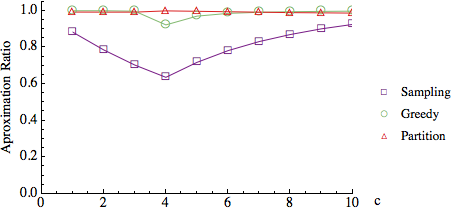
\includegraphics[width=0.8\textwidth]{images/l=25000,r=100000_Greedy_vs_Naive.png}
\caption{$|L|=25$k, $|R|=100$k, $d=20$, $a=1$}\label{fig:a=1:1}
\end{minipage}
\hspace{0cm}
\begin{minipage}[h]{0.48\textwidth}
\centering
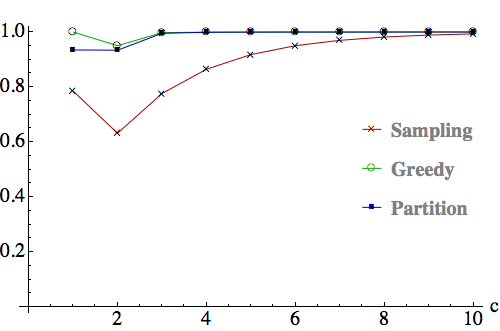
\includegraphics[width=0.8\textwidth]{images/l=50000,r=100000_Greedy_vs_Naive.png}
\caption{$|L|=50$k, $|R|=100$k, $d=20$, $a=1$}\label{fig:a=1:2}
\end{minipage}
\vspace{-0.2in}
\end{figure}


% Can we show the graph for larger c? Maybe up to 20?
% Also I can't believe that greedy is optimal. I am still tempted to say that
% greedy will do badly when d is small. Like d < 5.

\vs
In contrast to the case when $a=1$, the sampling algorithm performs
worse when $a>1$ but performs increasingly better with $c$ as
demonstrated by Figures~\ref{fig:a=2} and \ref{fig:a=4}. The greedy
algorithm continues to produce solutions that are nearly optimal,
regardless of the settings of $c$ and $a$. Therefore, our simulations
suggest that in many cases a software engineer can simply design the
sampling method for solving the $(c, a)$-recommendation subgraph
problem. In those cases where the sampling is not suitable as flagged by our analysis, 
we still find that the greedy performs adequately and is simple to implement.


\begin{figure}[t]
\centering
\begin{minipage}[h]{0.48\textwidth}
\centering
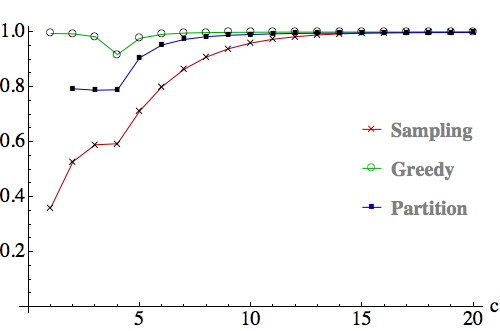
\includegraphics[width=0.8\textwidth]{images/l=50000,r=100000,a=2_Greedy_vs_Naive.png}
\caption{$|L|=50$k, $|R|=100$k, $d=20$, $a=2$}\label{fig:a=2}
\end{minipage}
\hspace{0cm}
\begin{minipage}[h]{0.48\textwidth}
\centering
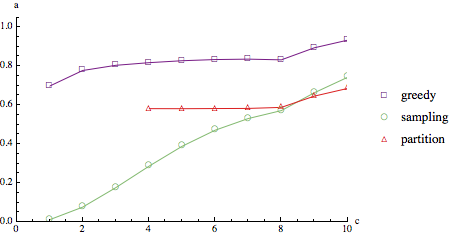
\includegraphics[width=0.8\textwidth]{images/l=50000,r=100000,a=4_Greedy_vs_Naive.png}
\caption{$|L|=50$k, $|R|=100$k, $d=20$, $a=4$}\label{fig:a=4}
\end{minipage}
\vspace{-0.2in}
\end{figure}

\vs
In short, our synthetic experiments show the following strengths of each algorithm:\\
\textbf{Sampling Algorithm:} This algorithm uses little to no memory and can
be implemented as an online algorithm. If keeping the underlying graph in
memory is an issue, then chances are this algorithm will do well while only needing
a fraction of the resources the other two algorithms would take.\\

\textbf{Partition Algorithm:} This algorithm does well, but only when $a$ is small. In this
realm, partition is not only competitive with greedy, but it's actually better. However
this performance comes at expense of significant runtime and space costs. This algorithm
will recover the  optimal solution when $a=1$, and will likely be able to recover a
good $(c,a)$-recommendation subgraph when we know that a perfect one exists. It also has
a distinct advantage over both greedy and sampling algorithms when $lc=ra$. \\

\textbf{Greedy Algorithm:} This algorithm is the all around best algorithm we tested.
It's runs really quickly because it only requires a single pass over the data and uses
relatively little amounts of space enabling it run completely in memory for graphs with
as many as tens of millions of edges. It's not as quick as sampling or accurate as partition
when $a$ is small, but it has great performance over all settings of parameters.